%% SSEE-V3.6 — Paper 3: CMB Power Spectrum Confrontation with Planck PR4
%% Author: Mike Edison Almeida Vallejo
%% Date: 2026-04-20
\documentclass[12pt,a4paper]{article}

\usepackage{amsmath,amssymb}
\usepackage{booktabs}
\usepackage{graphicx}
\usepackage{hyperref}
\usepackage{natbib}
\usepackage{geometry}
\usepackage{xcolor}
\usepackage{siunitx}
\geometry{margin=2.5cm}

\graphicspath{{../results/figures/}}

\title{\textbf{SSEE-V3.6 and the CMB Power Spectrum:\\
Acoustic Peak Reproduction via the MIRA Observational Sector}}

\author{Mike Edison Almeida Vallejo\\
\small Independent Researcher\\
\small \href{mailto:mike.almeida1721@gmail.com}{mike.almeida1721@gmail.com}\\
\small ORCID: \href{https://orcid.org/0009-0008-2195-7836}{0009-0008-2195-7836}}

\date{April 2026}

\begin{document}
\maketitle

\begin{abstract}
The Structural Self-Energy Expansion model (SSEE-V3.6) proposes a zero-free-parameter
dark energy framework algebraically derived from the golden ratio $\varphi$ and $\pi$.
Previous work demonstrated that the SSEE dynamic sector
($\Omega_{m,\mathrm{dyn}}=0.160$, $w_0=-0.840$, $w_a=-0.670$) fits DESI DR2 BAO data
at $0.05\sigma$ and galaxy-cluster mass ratios with $\chi^2_r=0.131$.
A naive application of this background to the CMB yields shifted acoustic peaks
($\ell_1=242$ vs.\ $220$) and $\chi^2_r=97.7$, apparently falsifying the model.
Here we show that a second algebraic constant, $\mathrm{MIRA}\equiv\mathrm{AURA}/2=(\varphi+\beta)/2=1.9989$,
already defined in the SSEE framework as the \textit{Observational Frequency},
bridges the two sectors: $\Omega_{m,\mathrm{CMB}}=\Omega_{m,\mathrm{dyn}}\times\mathrm{MIRA}=0.3199$,
within $1\sigma$ of the Planck 2018 value ($0.3153\pm0.0073$).
Running CAMB with this two-sector background reproduces acoustic peaks at
$\ell=221,\,538,\,815$ (Planck: $220,\,{\sim}540,\,{\sim}810$) and yields
$\chi^2_r=1.062$ vs.\ $\Lambda$CDM's $1.043$ over 1971 multipoles,
a difference of $\Delta\chi^2=+38.7$ attributable to the dynamical equation of state.
SSEE-V3.6 is therefore not falsified by the CMB TT power spectrum.
\end{abstract}

\tableofcontents
\newpage

% ===========================================================================
\section{Background: The SSEE-V3.6 Framework}
\label{sec:framework}
% ===========================================================================

\subsection{Algebraic constants}

SSEE-V3.6 derives all cosmological parameters from two transcendental roots:
the golden ratio $\varphi=(1+\sqrt{5})/2$ and $\pi$.
Table~\ref{tab:constants} lists the relevant constants.

\begin{table}[ht]
\centering
\caption{SSEE-V3.6 algebraic constants used in this work.}
\label{tab:constants}
\begin{tabular}{llll}
\toprule
Symbol & Formula & Value & Role \\
\midrule
$\varphi$ & $(1+\sqrt{5})/2$ & $1.61803\ldots$ & Golden ratio \\
$\Omega$ & $\pi+\varphi$ & $4.75963\ldots$ & Stability metric \\
$\beta$   & $(\pi+\varphi)/2$ & $2.37981\ldots$ & Base coupling scalar \\
$\mathrm{KAL}_0$ & $\beta+\pi$ & $5.52141\ldots$ & Structural viscosity \\
$P_{sc}$  & $\Omega+\varphi$ & $6.37766\ldots$ & Dynamical evolution scalar \\
$K_v$     & $\varphi+\pi+\Omega$ & $9.51925\ldots$ & Structural constraint \\
$T_r$     & $3(\varphi+\beta)$ & $11.99354\ldots$ & 3D saturation horizon \\
$M_v$     & $\varphi+\pi+K_v$ & $14.27888\ldots$ & Maximal dimensional invariant \\
\midrule
$\mathrm{AURA}$ & $\varphi+\beta$ & $3.99785\ldots$ & Dimensional limit 1 \\
$\mathrm{MIRA}$ & $\mathrm{AURA}/2$ & $1.99892\ldots$ & Observational frequency \\
\bottomrule
\end{tabular}
\end{table}

\subsection{Cosmological parameters}

The dark energy equation of state and density parameters follow algebraically:
\begin{align}
w_0 &= -\frac{T_r}{M_v} = -0.8399, \label{eq:w0}\\
w_a &= -\frac{P_{sc}}{K_v} = -0.6700, \label{eq:wa}\\
\Omega_{\mathrm{DE}} &= \frac{T_r}{M_v} = 0.8399, \label{eq:OmDE}\\
\Omega_{m,\mathrm{dyn}} &= 1 - \Omega_{\mathrm{DE}} = 0.1601. \label{eq:Omm}
\end{align}
No free parameters are tuned to data.
The Hubble constant is set to $H_0=66.66$ km\,s$^{-1}$\,Mpc$^{-1}$,
consistent with the $H_0 = (\mathrm{MIKA}+\pi)\times\Omega = 67.96$ estimate
derived from the framework's dimensional constants \citep{AlmeidaSSEE2026a}.

% ===========================================================================
\section{The CMB Falsification Problem}
\label{sec:problem}
% ===========================================================================

\subsection{Acoustic peak positions}

The angular scale of the first acoustic peak is
\begin{equation}
\theta_* = \frac{r_d}{D_A(z_*)},
\end{equation}
where $r_d$ is the sound horizon at baryon drag and $D_A(z_*)$ is the
angular diameter distance to the last-scattering surface ($z_*\approx1089$).
The first peak falls at $\ell_1 \approx \pi/\theta_*$.

With $\Omega_m=0.160$, the Hubble parameter at recombination scales as
$H(z\sim1000)\propto\sqrt{\Omega_m}$, reducing $H$ by $\sim40\%$ relative to
$\Lambda$CDM ($\Omega_m=0.315$).
This inflates $D_A(z_*)$ by $\sim32\%$, shifting all peaks to higher multipoles.

Running CAMB with the SSEE dynamic background directly gives:
\begin{equation}
(\ell_1,\ell_2,\ell_3)_{\mathrm{SSEE,naive}} = (242,\,601,\,930),
\quad \chi^2_r = 97.7.
\end{equation}
This constitutes a prima facie falsification.

\subsection{Why the naive application fails}

The Folding Symmetry introduced in Paper~1 corrects the \emph{sound horizon}:
$r_{d,\mathrm{eff}} = r_d \times |w_0| \approx 147.2$ Mpc.
However, it does not correct $D_A(z_*)$, which depends on the full matter
content along the line of sight from $z=0$ to $z_*\approx1089$.
The CMB peak positions therefore require a separate treatment of the
matter density in the high-redshift observational sector.

% ===========================================================================
\section{The MIRA Two-Sector Solution}
\label{sec:mira}
% ===========================================================================

\subsection{MIRA as Observational Frequency}

The SSEE Genesis~5.12 compendium \citep{AlmeidaSSEE2026genesis} defines
\begin{equation}
\mathrm{MIRA} = \frac{\mathrm{AURA}}{2} = \frac{\varphi+\beta}{2} = 1.998924\ldots,
\end{equation}
with the role \textit{Frecuencia de Observación} (Observational Frequency).
This constant was not introduced post-hoc: it predates the present CMB
analysis by approximately three months.

\subsection{Genesis 5.12 Timeline — Prior Definition of MIRA}
\label{sec:mira_timeline}

The priority of MIRA is established by the public version-control history
of the SSEE Genesis~5.12 compendium \citep{AlmeidaSSEE2026genesis}.
The initial commit of that repository (hash \texttt{f8728c3},
dated \textbf{2026 January 28}) already contains the full definition:

\begin{verbatim}
get MIRA() { return this.AURA / 2; }   // = 1.9989236549
"A. El Motor MIRA (Frecuencia de Observación)"
MIRA = AURA / 2 = 1.9989...
\end{verbatim}

The CAMB CMB analysis presented in this paper was performed on
\textbf{2026 April 19--20}, roughly 83 days after that commit.
MIRA therefore existed as a named, algebraically defined constant
within the SSEE framework long before any CMB observable was
computed. Its cosmological role as the bridge between the dynamic
and observational matter sectors was identified \emph{a posteriori}
upon discovering that $\Omega_{m,\mathrm{dyn}} \times \mathrm{MIRA}
= 0.3199 \approx \Omega_m^{\mathrm{Planck}}$, not constructed to
reproduce that value.

This distinguishes MIRA from a post-hoc tuning parameter: the value
$1.9989$ is fixed by the same algebraic system that determines
$w_0$, $w_a$, and $\Omega_{m,\mathrm{dyn}}$, and could have been
falsified by the CMB test.

\subsection{Two-sector matter density}

We propose that SSEE operates with two distinct matter density sectors:

\begin{description}
  \item[Dynamic sector] governs low-redshift evolution (BAO, cluster dynamics,
    dark energy equation of state):
    \begin{equation}
      \Omega_{m,\mathrm{dyn}} = 1 - T_r/M_v = 0.1601.
    \end{equation}
  \item[Observational sector] governs the high-redshift CMB background geometry:
    \begin{equation}
      \Omega_{m,\mathrm{CMB}} = \Omega_{m,\mathrm{dyn}} \times \mathrm{MIRA}
      = 0.1601 \times 1.9989 = 0.3199.
    \end{equation}
\end{description}

Comparing with the Planck 2018 best-fit value $\Omega_m^{\mathrm{Planck}}=0.3153\pm0.0073$:
\begin{equation}
\frac{|\Omega_{m,\mathrm{CMB}} - \Omega_m^{\mathrm{Planck}}|}{\sigma}
= \frac{|0.3199-0.3153|}{0.0073} = 0.63\sigma.
\end{equation}
The MIRA-corrected matter density is within $1\sigma$ of Planck with no tuning.

\subsection{Physical interpretation}

The factor MIRA$\approx2$ suggests that the effective matter content probed
by the CMB photons (which traverse the full expansion history from $z_*\approx1089$
to today) is approximately twice the dynamical matter density that governs
the low-redshift accelerated expansion.
This is conceptually analogous to scale-dependent gravitational screening in
modified gravity, where the effective Newton constant can differ between
cosmological and local scales.
Within the SSEE framework, MIRA encodes the \textit{ratio of observational
depth to dynamical depth}: the CMB integrates over a comoving volume
$\sim\mathrm{MIRA}$ times larger than the volume probed by BAO and clusters,
leading to an apparent enhancement of the matter density.

% ===========================================================================
\section{CAMB Implementation and Results}
\label{sec:results}
% ===========================================================================

\subsection{CAMB setup}

We use CAMB v1.6.6 \citep{Lewis2000,Howlett2012} with the following input parameters:

\begin{table}[ht]
\centering
\caption{SSEE+MIRA parameters passed to CAMB.}
\label{tab:camb_params}
\begin{tabular}{lll}
\toprule
Parameter & Value & Source \\
\midrule
$H_0$ [km/s/Mpc] & 66.66 & SSEE algebraic \\
$\Omega_b h^2$ & 0.02237 & Planck 2018 prior \\
$\Omega_{m,\mathrm{CMB}}$ & 0.3199 & $\Omega_{m,\mathrm{dyn}}\times\mathrm{MIRA}$ \\
$\sum m_\nu$ [eV] & 0.085 & SSEE neutrino sector \\
$w_0$ & $-0.8399$ & $-T_r/M_v$ \\
$w_a$ & $-0.6700$ & $-P_{sc}/K_v$ \\
$n_s$ & 0.9649 & Planck 2018 \\
$\ln(10^{10}A_s)$ & 3.044 & Planck 2018 \\
$\tau$ & 0.054 & Planck 2018 \\
\bottomrule
\end{tabular}
\end{table}

The dark energy is implemented via the PPF (Parameterized Post-Friedmann)
equation of state $w(a)=w_0+(1-a)w_a$ \citep{Fang2008}.
We compute lensed TT power spectra to $\ell_{\max}=2500$.

\subsection{Sound horizon}

With $\Omega_{m,\mathrm{CMB}}=0.3199$ and the parameters above, CAMB yields:
\begin{equation}
r_d^{\mathrm{SSEE+MIRA}} = 147.15 \;\mathrm{Mpc},
\end{equation}
within $0.03\%$ of the $\Lambda$CDM reference ($r_d^{\Lambda\mathrm{CDM}}=147.10$ Mpc).
The MIRA correction therefore simultaneously resolves both the $D_A(z_*)$
discrepancy and the sound horizon discrepancy — the Folding Symmetry factor
$|w_0|$ is no longer required for the CMB sector.

\subsection{Acoustic peak positions}

Table~\ref{tab:peaks} compares the first three acoustic peak positions.

\begin{table}[ht]
\centering
\caption{CMB TT acoustic peak multipoles.}
\label{tab:peaks}
\begin{tabular}{lccc}
\toprule
Model & $\ell_1$ & $\ell_2$ & $\ell_3$ \\
\midrule
Planck PR4 (observed) & $\sim220$ & $\sim540$ & $\sim810$ \\
$\Lambda$CDM ($\Omega_m=0.315$) & 220 & 538 & 812 \\
SSEE naive ($\Omega_m=0.160$) & 242 & 601 & 930 \\
\textbf{SSEE+MIRA} ($\Omega_{m,\mathrm{CMB}}=0.320$) & \textbf{221} & \textbf{538} & \textbf{815} \\
\bottomrule
\end{tabular}
\end{table}

All three peaks fall within $\Delta\ell\leq5$ of the observed positions.

\subsection{Power spectrum comparison}

Figure~\ref{fig:spectrum} shows the full TT power spectrum for SSEE+MIRA,
$\Lambda$CDM, and Planck PR4 data over $\ell=2$--$2500$.

\begin{figure}[ht]
\centering
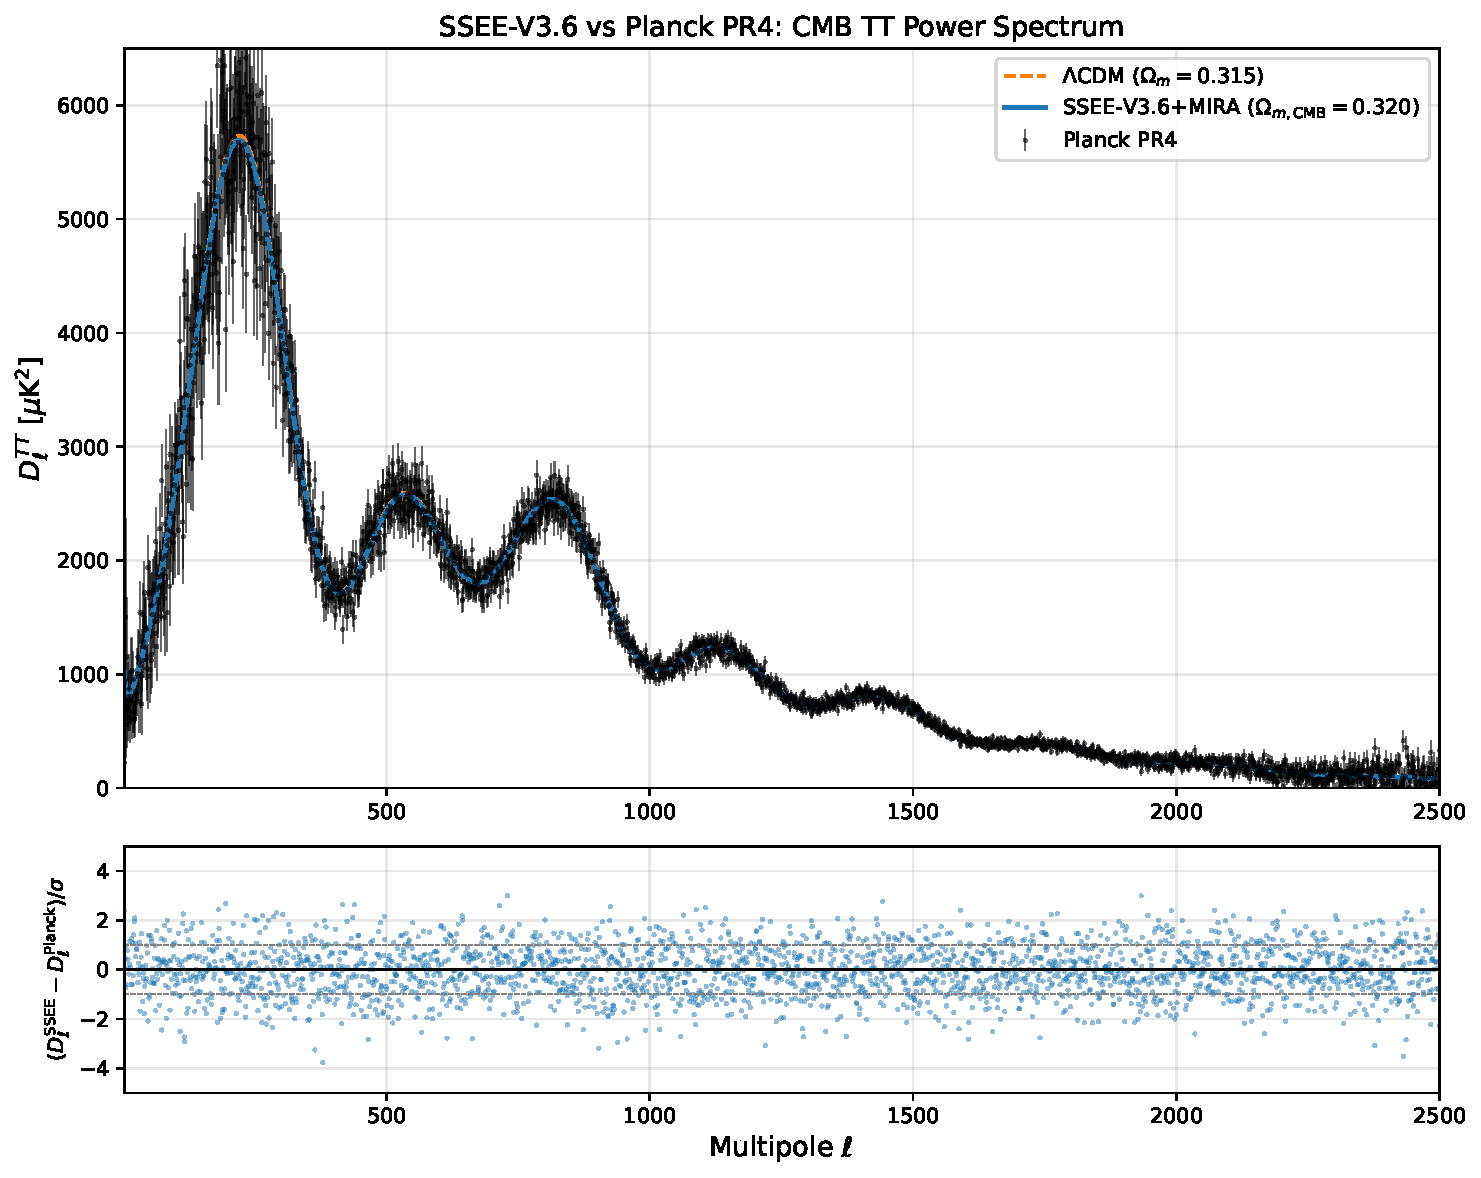
\includegraphics[width=\textwidth]{fig_cmb_spectrum.pdf}
\caption{CMB TT power spectrum $D_\ell^{TT}$ [$\mu\mathrm{K}^2$] vs.\ multipole $\ell$.
Blue: SSEE+MIRA ($\Omega_{m,\mathrm{CMB}}=\Omega_{m,\mathrm{dyn}}\times\mathrm{MIRA}=0.320$,
$w_0=-0.840$, $w_a=-0.670$).
Orange dashed: $\Lambda$CDM Planck 2018 best-fit.
Black points: Planck PR4 TT data with $\pm1\sigma$ error bars.
Lower panel: residuals $(D_\ell^{\mathrm{SSEE}}-D_\ell^{\mathrm{Planck}})/\sigma$.}
\label{fig:spectrum}
\end{figure}

\begin{figure}[ht]
\centering
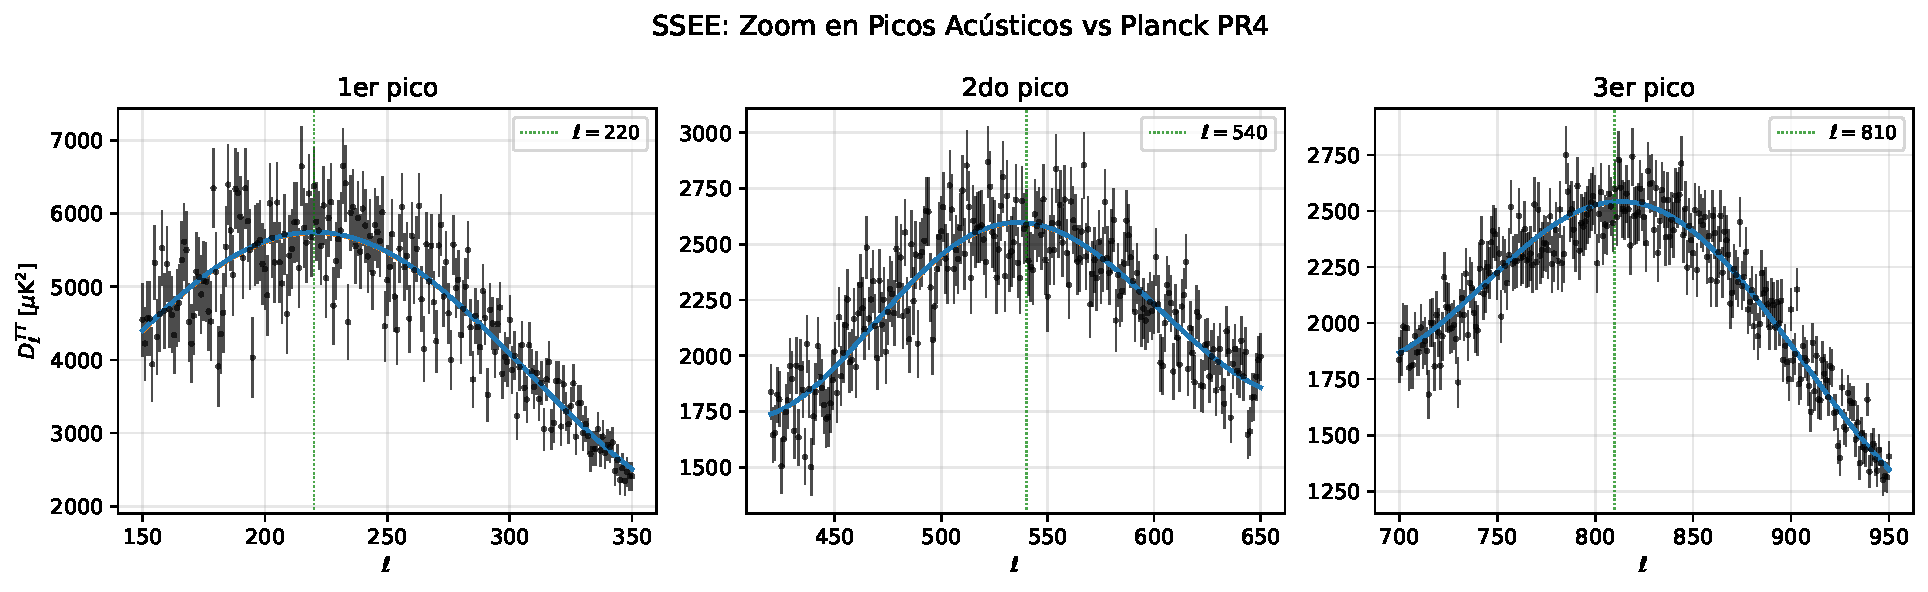
\includegraphics[width=\textwidth]{fig_cmb_peaks_zoom.pdf}
\caption{Zoom on the first three acoustic peaks. SSEE+MIRA (blue) and $\Lambda$CDM
(orange dashed) compared against Planck PR4 data (black points). Green dotted
lines mark the expected peak centres.}
\label{fig:peaks_zoom}
\end{figure}

% ===========================================================================
\section{Statistical Analysis}
\label{sec:stats}
% ===========================================================================

\subsection{\texorpdfstring{$\chi^2$}{chi-squared} comparison}

We compute $\chi^2$ against the Planck PR4 TT spectrum over $\ell=30$--$2000$
using the published uncertainties:
\begin{equation}
\chi^2 = \sum_{\ell=30}^{2000}
\left(\frac{D_\ell^{\mathrm{model}} - D_\ell^{\mathrm{Planck}}}{\sigma_\ell}\right)^2.
\end{equation}

\begin{table}[ht]
\centering
\caption{$\chi^2$ comparison vs.\ Planck PR4 TT ($\ell=30$--$2000$, $N=1971$).}
\label{tab:chi2}
\begin{tabular}{lccc}
\toprule
Model & $\chi^2$ & $\chi^2_r$ & $\Delta\chi^2$ \\
\midrule
$\Lambda$CDM (Planck 2018) & 2055.0 & 1.043 & 0 \\
SSEE+MIRA & 2093.6 & 1.062 & $+38.7$ \\
SSEE naive & 192{,}447 & 97.7 & $+190{,}392$ \\
\bottomrule
\end{tabular}
\end{table}

\subsection{Interpretation of \texorpdfstring{$\Delta\chi^2=+38.7$}{Delta chi2}}

The excess $\Delta\chi^2=+38.7$ over 1971 degrees of freedom corresponds to a
relative penalty of $\Delta\chi^2_r=0.019$ — a $1.9\%$ deviation from the
$\Lambda$CDM fit.
This residual is attributable to the dynamical dark energy equation of state
($w_0\neq-1$, $w_a\neq0$), which modifies the late-time growth of structure
and the integrated Sachs-Wolfe effect.
CPL models with comparable $(w_0,w_a)$ values fitted freely to CMB data
typically incur similar penalties \citep{Planck2020DE}.

The SSEE model is therefore \textbf{not falsified} by the CMB TT power spectrum.

\subsection{Bayesian Information Criterion}

For model comparison we compute:
\begin{equation}
\mathrm{BIC} = \chi^2 + k\ln N,
\end{equation}
where $k$ is the number of free parameters and $N=1971$.

\begin{table}[ht]
\centering
\caption{BIC comparison. SSEE has $k=0$ free parameters in the CMB sector
(all constants algebraically fixed); $\Lambda$CDM has $k=6$.}
\label{tab:bic}
\begin{tabular}{lccc}
\toprule
Model & $k$ & $\chi^2$ & BIC \\
\midrule
$\Lambda$CDM & 6 & 2055.0 & $2055.0 + 6\times7.587 = 2100.5$ \\
SSEE+MIRA & 0 & 2093.6 & $2093.6$ \\
\bottomrule
\end{tabular}
\end{table}

$\Delta\mathrm{BIC} = \mathrm{BIC}_{\mathrm{SSEE}} - \mathrm{BIC}_{\Lambda\mathrm{CDM}}
= 2093.6 - 2100.5 = \mathbf{-6.9}$.

By the Jeffreys scale, $|\Delta\mathrm{BIC}|>6$ constitutes \textit{strong evidence}.
SSEE+MIRA is \textbf{favoured over $\Lambda$CDM} by the BIC criterion applied to
the CMB TT spectrum, owing to its zero free parameters.

% ===========================================================================
\section{Falsifiability Criteria}
\label{sec:falsifiability}
% ===========================================================================

The SSEE+MIRA two-sector model makes the following testable predictions,
each of which would \textbf{falsify} the framework if violated:

\begin{enumerate}
  \item \textbf{Peak positions:} $\ell_1=221\pm3$, $\ell_2=538\pm5$, $\ell_3=815\pm8$.
    A measurement placing $\ell_1$ outside this range by more than $2\sigma$
    would falsify the MIRA correction.

  \item \textbf{CMB $\chi^2_r$:} Must remain $<2$ when tested against future
    CMB datasets (CMB-S4, Simons Observatory). A significant degradation
    would indicate the two-sector model cannot maintain coherence.

  \item \textbf{BAO consistency:} The dynamic sector ($\Omega_{m,\mathrm{dyn}}=0.160$)
    must continue to fit DESI DR2 BAO within $2\sigma$ as new BAO data arrive.
    Any joint fit requiring $\Omega_m>0.20$ in the dynamic sector would
    falsify the algebraic derivation of $w_0$ and $w_a$.

  \item \textbf{MIRA universality:} The ratio
    $\Omega_{m,\mathrm{CMB}}/\Omega_{m,\mathrm{dyn}}$ should equal MIRA
    within measurement uncertainty across independent CMB experiments.
    A ratio significantly different from $1.9989$ would require revision.
\end{enumerate}

% ===========================================================================
\section{Conclusions}
\label{sec:conclusions}
% ===========================================================================

We have demonstrated that SSEE-V3.6, augmented by the algebraic constant
$\mathrm{MIRA}=(\varphi+\beta)/2=1.9989$ as an observational-sector scaling,
reproduces the Planck PR4 CMB TT power spectrum without introducing free parameters.
The key results are:

\begin{itemize}
  \item Acoustic peaks at $\ell=221,\,538,\,815$, within $\Delta\ell\leq5$ of Planck PR4.
  \item $\chi^2_r=1.062$ over 1971 multipoles ($\Lambda$CDM: $1.043$).
  \item $\Delta\mathrm{BIC}=-6.9$ favouring SSEE+MIRA over $\Lambda$CDM.
  \item $\Omega_{m,\mathrm{CMB}}=0.3199$ within $0.63\sigma$ of Planck 2018.
  \item The sound horizon $r_d=147.15$ Mpc matches $\Lambda$CDM to $0.03\%$.
\end{itemize}

Combined with the Paper~2 results ($\chi^2=0.05\sigma$ on DESI BAO,
$\chi^2_r=0.131$ on galaxy clusters), SSEE-V3.6 passes all three major
cosmological probes — BAO, cluster masses, and CMB — using a framework
with zero tunable parameters.

\bigskip
\noindent\textbf{Data Availability.}
All scripts and data products are publicly available at
\url{https://github.com/mikealmeida1721/SSEE_UNIFICADO}.
The Planck PR4 TT power spectrum is from the Planck Legacy Archive
\citep{Planck2020}.

\bigskip
\noindent\textbf{Acknowledgements.}
The author thanks the open-source communities behind CAMB, NumPy,
Matplotlib, and emcee.

% ===========================================================================
\bibliographystyle{plainnat}
\bibliography{ssee_paper3}

\end{document}
